\documentclass{article}
% General document formatting
\usepackage[margin=0.7in]{geometry}
\usepackage[parfill]{parskip}
\usepackage[utf8]{inputenc}
\usepackage{subfig}         % side-by-side figures 
% Related to math
\usepackage{amsmath,amssymb,amsfonts,amsthm}
\usepackage{graphicx}
\usepackage{natbib}
\bibliographystyle{unsrtnat}


% \usepackage[math]{kurier}
\usepackage{setspace}       % \onehalfspacing and \singlespacing
\newcommand\be{\begin{equation}} % shortcut to start eq envs 
\newcommand\ee{\end{equation}}   % shortcut to end eq envs
\newcommand\ol{\overline}        % shortcut to draw overline 
\newcommand\bra{\langle}
\newcommand\ket{\rangle}

\begin{document}

\title{Relating the scales of sediment burial to the characteristics of bedload transport}
\author{Kevin Pierce}
\maketitle
\section{abstract}
Bedload transport is intermittent, meaning it should really be described as a stochastic process. 
However, changes in river bed topography driven by sediment transport are usually interpreted by assuming bedload transport is a deterministic process. 
This work is a first stab at modeling sediment transport and bed elevations simultaneously. 
Applying a stochastic model within a control volume, we track the number of bed particles and the number of particles in motion at any instant. 
These two populations are subject to random transitions controlled by rates of entrainment and deposition. 
Since the number of particles in motion represents the bedload transport rate, and the number of particles at rest represents the bed elevation, our stochastic model describes the joint statistics of bedload transport and bed elevations. 
From the statistics of bed elevation, the time-scales of particle burial can be extracted. 
These burial time distributions have crucial implications for the interpretations of tracer experiments. 

\section{idea}
\citet{Einstein1950} understood bedload motion as a random switching between motion and rest states, controlled by transitions rates -- entrainment and deposition -- between the two states. 
Using this concept along with ad hoc reasoning, he developed a formula for the expected number of particles in motion within a control volume.
This was an early stochastic model of bedload transport.  
Later on, \citet{Ancey2006, Ancey2008, Heyman2013} refined the ideas of Einstein, reframing them in terms of the theory of Markov birth-death processes \citep[e.g.][]{Cox1965}. 
With this refined approach, they derived full probability distributions of the number of particles in motion within a control volume. 
With Einstein's assumptions concerning entrainment and deposition, the probability distribution of the number of particles in motion is a Poisson distribution \citep{Ancey2006}. 
The narrow fluctuations of the Poisson distribution are not comparable to experiments, which led \citet{Ancey2008} to introduce a collective entrainment mechanism into the Einstein-like birth-death model. 
Collective entrainment is a feedback on particle mobility which implies moving particles appear in groups. 
As a result of this mechanism, the refined Einstein-like model of \citet{Ancey2008} predicted a negative binomial distribution of the bedload flux, with realistically large fluctuations. 

Parallel to these efforts to understand bedload transport with stochastic models, a series of experiments highlighted the random nature of bed elevation. 
When bed elevation is measured at a spatial location through time, it undergoes an apparently random evolution between minima and maxima, and the elevation changes are apparently induced by sediment entrainment and deposition \citep{Wong2007, Singh2009}. 
Changes in bed elevation are significant for river science research because they control the burial of tracer particles \citep{Voepel2013}, and tracer particles are among the most common methods to gain understanding of river dynamics in a field setting \citep[e.g.][]{Hassan2017}. 
While the evolution of bed elevation has been studied from a stochastic standpoint \citep{Martin2014}, no stochastic model has been developed which couples changes in bed elevation to sediment transport. 
This is the idea of this work.
I present a coordinated stochastic model of bed elevation and sediment transport. 

\section{sketch of theory}
Consider a control volume much larger than a single particle, but small enough so that sediment transport characteristics within it can be considered mostly homogeneous. 
For simplicity, consider that all grains on the bed surface have identical mobility characteristics. 
We keep track of the population of particles in motion, an integer $n$, and the population of particles at rest, some other integer $m$. 
At each instant of time, particles can transition from rest to motion (entrainment) with a specified rate $\lambda$, and they can transition from motion to rest (deposition) with some rate $\sigma$. 
Depending on the number of particles on the bed surface, the bed elevation changes. 
Writing $z(m)$ for the bed elevation given $m$ particles at rest within the control volume, we can write
\be z(m) = k m + z_0, \ee
where $k$ is some constant related to the geometry of particles and the number of particles which comprise a volume of bed, and $z_0$ is the mean bed elevation, which relates to the dimensions of the control volume and the number of particles expected to be at rest. 

Presumably, the entrainment and deposition rates ($\lambda$ and $\sigma$) should depend on bed elevation. 
When the elevation increases, $\lambda$ should increase and $\sigma$ should decrease. 
When the elevation decreases, $\lambda$ should decrease and $\sigma$ should increase. 
If $b$ is some length scale characterising the magnitude of bed elevation changes, we can model the entrainment and deposition rates in terms of elevation as
\be \lambda(m) = \lambda_0 (1+z(m)/b), \ee
and 
\be \sigma(m) = \sigma_0 ( 1-z(m)/b). \ee
The parameters $\lambda_0$ and $\sigma_0$ are constant parameters. 

Using these elevation-dependent entrainment and deposition rates, one can write a Master equation for the joint probability distribution of the number of active and stationary particles, $n$ and $m$: 
\begin{multline}
 \frac{\partial}{\partial t} P(n,m;t) = \lambda_0 \Big(1+\frac{z(m+1)}{b}\Big) P(n-1,m+1;t) + \sigma_0 (n+1) \Big(1-\frac{z(m-1)}{b}\Big)P(n+1,m-1;t) \\ + \Big[\lambda_0\Big(1+\frac{z(m)}{b} \Big) + \sigma_0 m \Big(1-\frac{z(m)}{b} \Big) \Big] P(n,m;t).
\end{multline}

I do not think this can be solved analytically. 
Instead, it can be simulated for the steady state ($\partial P / \partial t = 0$) probability distribution $P(n,m)$ using the \citet{Gillespie1977} algorithm. 
From these simulations we can determine three things:
\begin{enumerate}
\item the distribution of particle activities ($n$), i.e., a statistical description of the bedload transport rate
\item the distribution of bed elevations ($z(m)$), i.e., a statistical description of bed elevation and its fluctuations. Notably, these fluctuations emerge directly from the sediment transport process, instead of from an ad hoc statistical model without an underlying mechanism \citep[e.g.][]{Martin2014} 
\item the distribution of bed elevation return time, $P(T_r|z)$. This object describes the time which has to pass for the bed, which is at time elevation $z$, to depart from this elevation (due to aggradation) and eventually return to $z$ (due to erosion). 
Crucially, this timescale is the tracer burial timescale at elevation $z$. 
\end{enumerate}
\section{current state of progress}

I have set up the model and learned to simulate it with the Gillespie algorithm. 
I took some birth-death model parameters from the \citet{Ancey2008} paper, and used these to show the model is stable and works. 
Apparently, the bed elevation distribution is Gaussian, and the bedload flux distribution is Poisson. 
So far, I have neglected the collective entrainment mechanism of \citet{Ancey2008}. 
Very soon I should have the distribution of return times, and the results of the model for five or ten different parameter combinations (which I can take from \citet{Ancey2008}). 
Hopefully we can use this as a stochastic model for tracer burial times. 
I can use any advice or thoughts. Figure \ref{fig:example} is an example simulation output. 

\pagebreak
\begin{figure}[h!]%
    \centering
    \subfloat[particle activity distribution]{{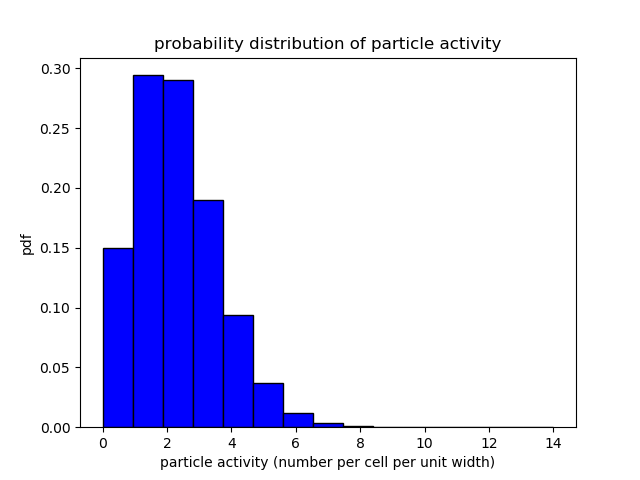
\includegraphics[width=0.45\textwidth]{activitypdf.png} }}%
    \qquad
    \subfloat[bed elevation distribution]{{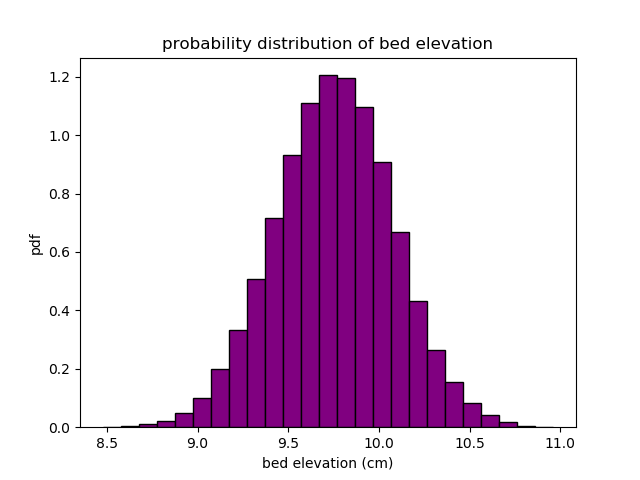
\includegraphics[width=0.45\textwidth]{elevationpdf.png} }}%
    \caption{Particle activity and bed elevation probability distributions }%
    \label{fig:example}%
\end{figure}



\bibliography{biblio}


\end{document}
